\documentclass[%
 reprint,
 amsmath,amssymb,
 aps,
]{revtex4-2}

\usepackage{graphicx}
\usepackage{dcolumn}
\usepackage{bm}
\usepackage[breaklinks, hidelinks, colorlinks=true,linkcolor=blue,citecolor=blue]{hyperref}

\begin{document}

\title{Detecção de Objetos Usando Mapas de Ativação em Redes Neurais Convolucionais}

\author{Wesley Nogueira Galvão}
\affiliation{Universidade Federal de São Carlos}

\date{\today}

\begin{abstract}
Neste trabalho, exploramos a detecção de objetos em imagens utilizando mapas de ativação de redes neurais convolucionais, com foco na localização de cães em imagens onde ocupam uma pequena parte da cena. Foram utilizados modelos ResNet18 e ResNet50, tanto pré-treinados no ImageNet quanto refinados no Oxford Pets. Os resultados qualitativos mostram o potencial do método para identificar regiões de interesse mesmo em cenários desafiadores.
\end{abstract}

\maketitle

\section{Introdução}
A detecção de objetos é uma tarefa fundamental em visão computacional. Métodos baseados em mapas de ativação de redes neurais profundas permitem identificar regiões relevantes em imagens, mesmo quando o objeto de interesse ocupa uma pequena área. Este trabalho investiga a aplicação de mapas de ativação para localizar cães em imagens genéricas, utilizando variantes da arquitetura ResNet.

\subsection{Motivação}
O uso de mapas de ativação é importante pois permite interpretar e visualizar quais regiões da imagem contribuem para a decisão do modelo, sendo útil em aplicações onde a localização precisa do objeto é relevante, como monitoramento, robótica e análise de imagens médicas.

\section{Objetivos}
\begin{enumerate}
    \item Avaliar a capacidade de modelos ResNet em localizar cães em imagens onde o animal ocupa uma pequena parte da cena.
    \item Comparar o desempenho de modelos treinados do zero, pré-treinados e refinados.
    \item Discutir qualitativamente os resultados obtidos.
\end{enumerate}

\section{Metodologia}
\subsection{Coleta de Dados}
Foram coletadas 10 imagens da internet contendo cães em diferentes cenários, garantindo que o animal não ocupasse a maior parte da imagem.

\subsection{Modelos Utilizados}
Foram empregados os modelos ResNet18 e ResNet50, nas seguintes variantes:
\begin{itemize}
    \item Pré-treinados no ImageNet
    \item Refinados (fine-tuned) no Oxford Pets
\end{itemize}

\subsection{Procedimento Experimental}
\begin{enumerate}
    \item As imagens foram redimensionadas para $2 \times 224 \times 2 \times 224$ pixels.
    \item As ativações da última camada convolucional antes do pooling global foram extraídas.
    \item A posição do valor máximo no mapa de ativação (tamanho $14 \times 14$) foi detectada.
    \item A posição correspondente foi mapeada para a imagem original.
    \item O procedimento foi repetido para todas as variantes dos modelos.
\end{enumerate}

\subsection{Implementação}
O código foi implementado em Python, utilizando PyTorch e torchvision. Os notebooks documentam todo o pipeline, desde o download dos dados, treinamento/refinamento dos modelos, até a extração e visualização dos mapas de ativação.

\section{Resultados}
Os resultados qualitativos mostram que:
\begin{itemize}
    \item Modelos pré-treinados no ImageNet conseguem localizar regiões de interesse, mas nem sempre coincidem com o cão.
    \item Modelos refinados no Oxford Pets apresentam melhor desempenho na localização do animal, mesmo em imagens desafiadoras.
    \item A ResNet50, por ser mais profunda, tende a produzir mapas de ativação mais focados.
\end{itemize}

\begin{figure}
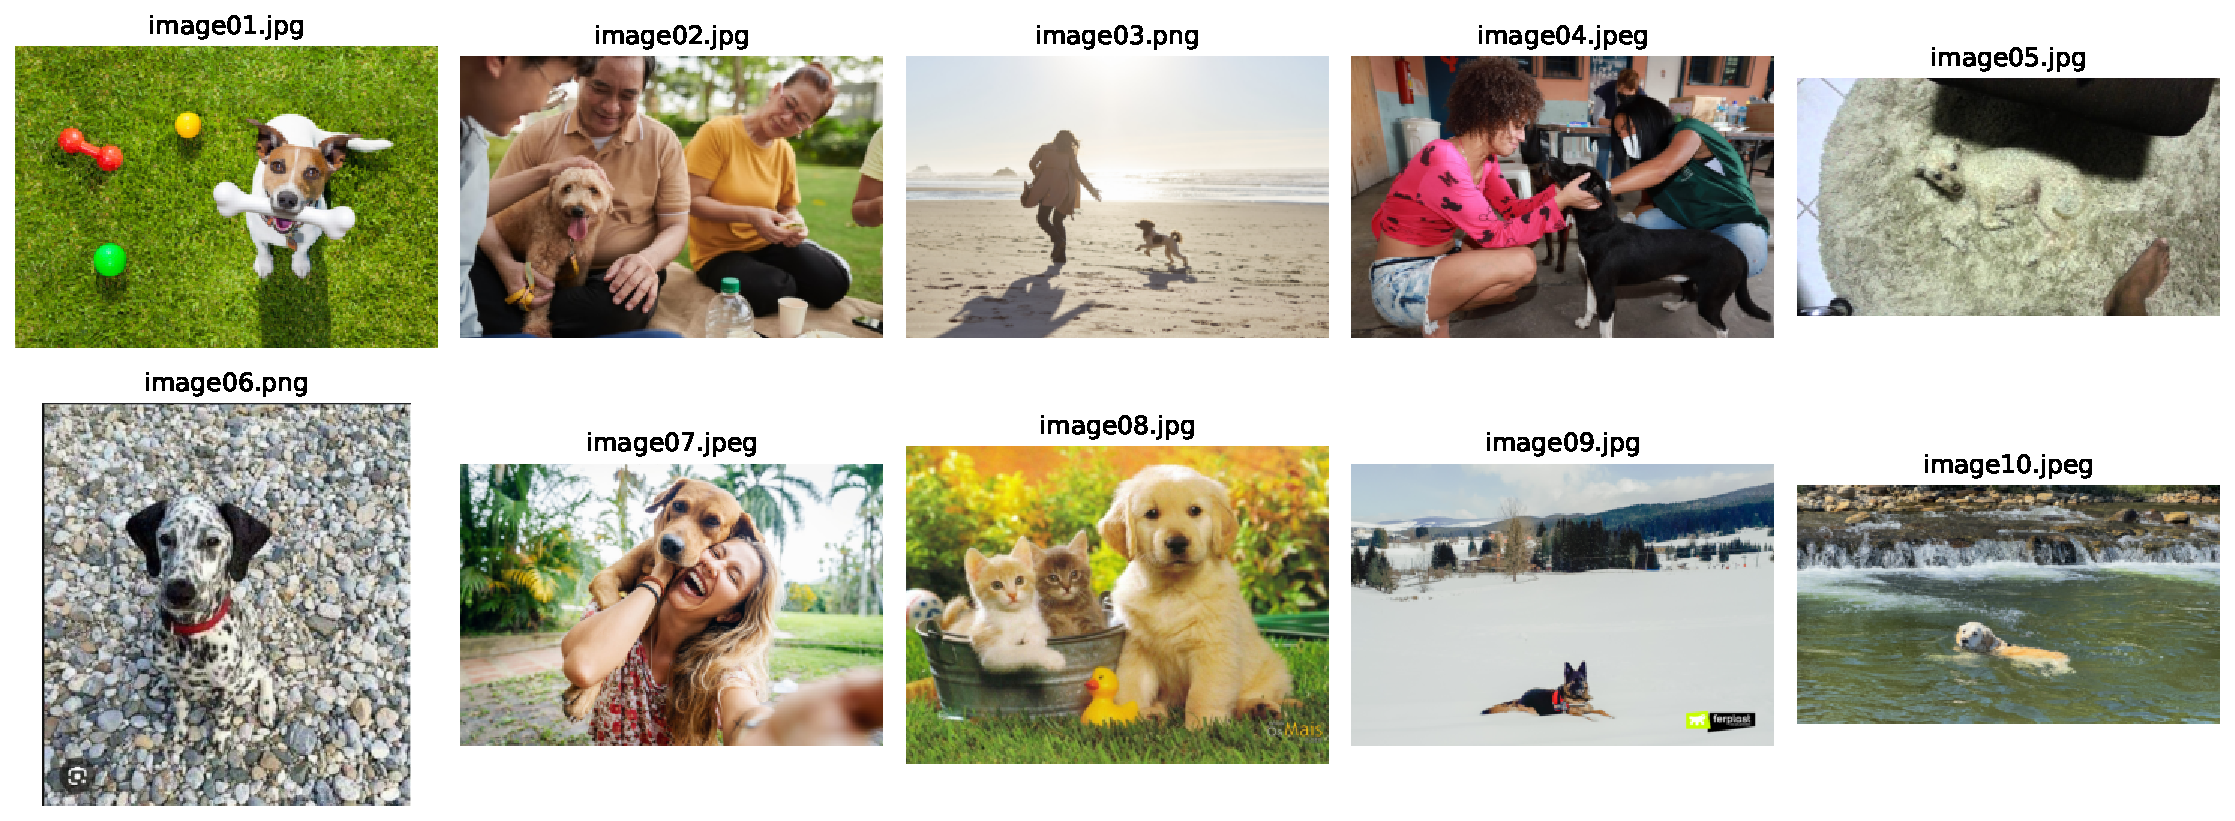
\includegraphics[width=\columnwidth]{imgs/dogs_image_grid.pdf}
\caption{Exemplo das imagens utilizadas nos experimentos.}
\end{figure}

% Figura de página inteira (largura total)
\begin{figure*}[htb]
    \centering
    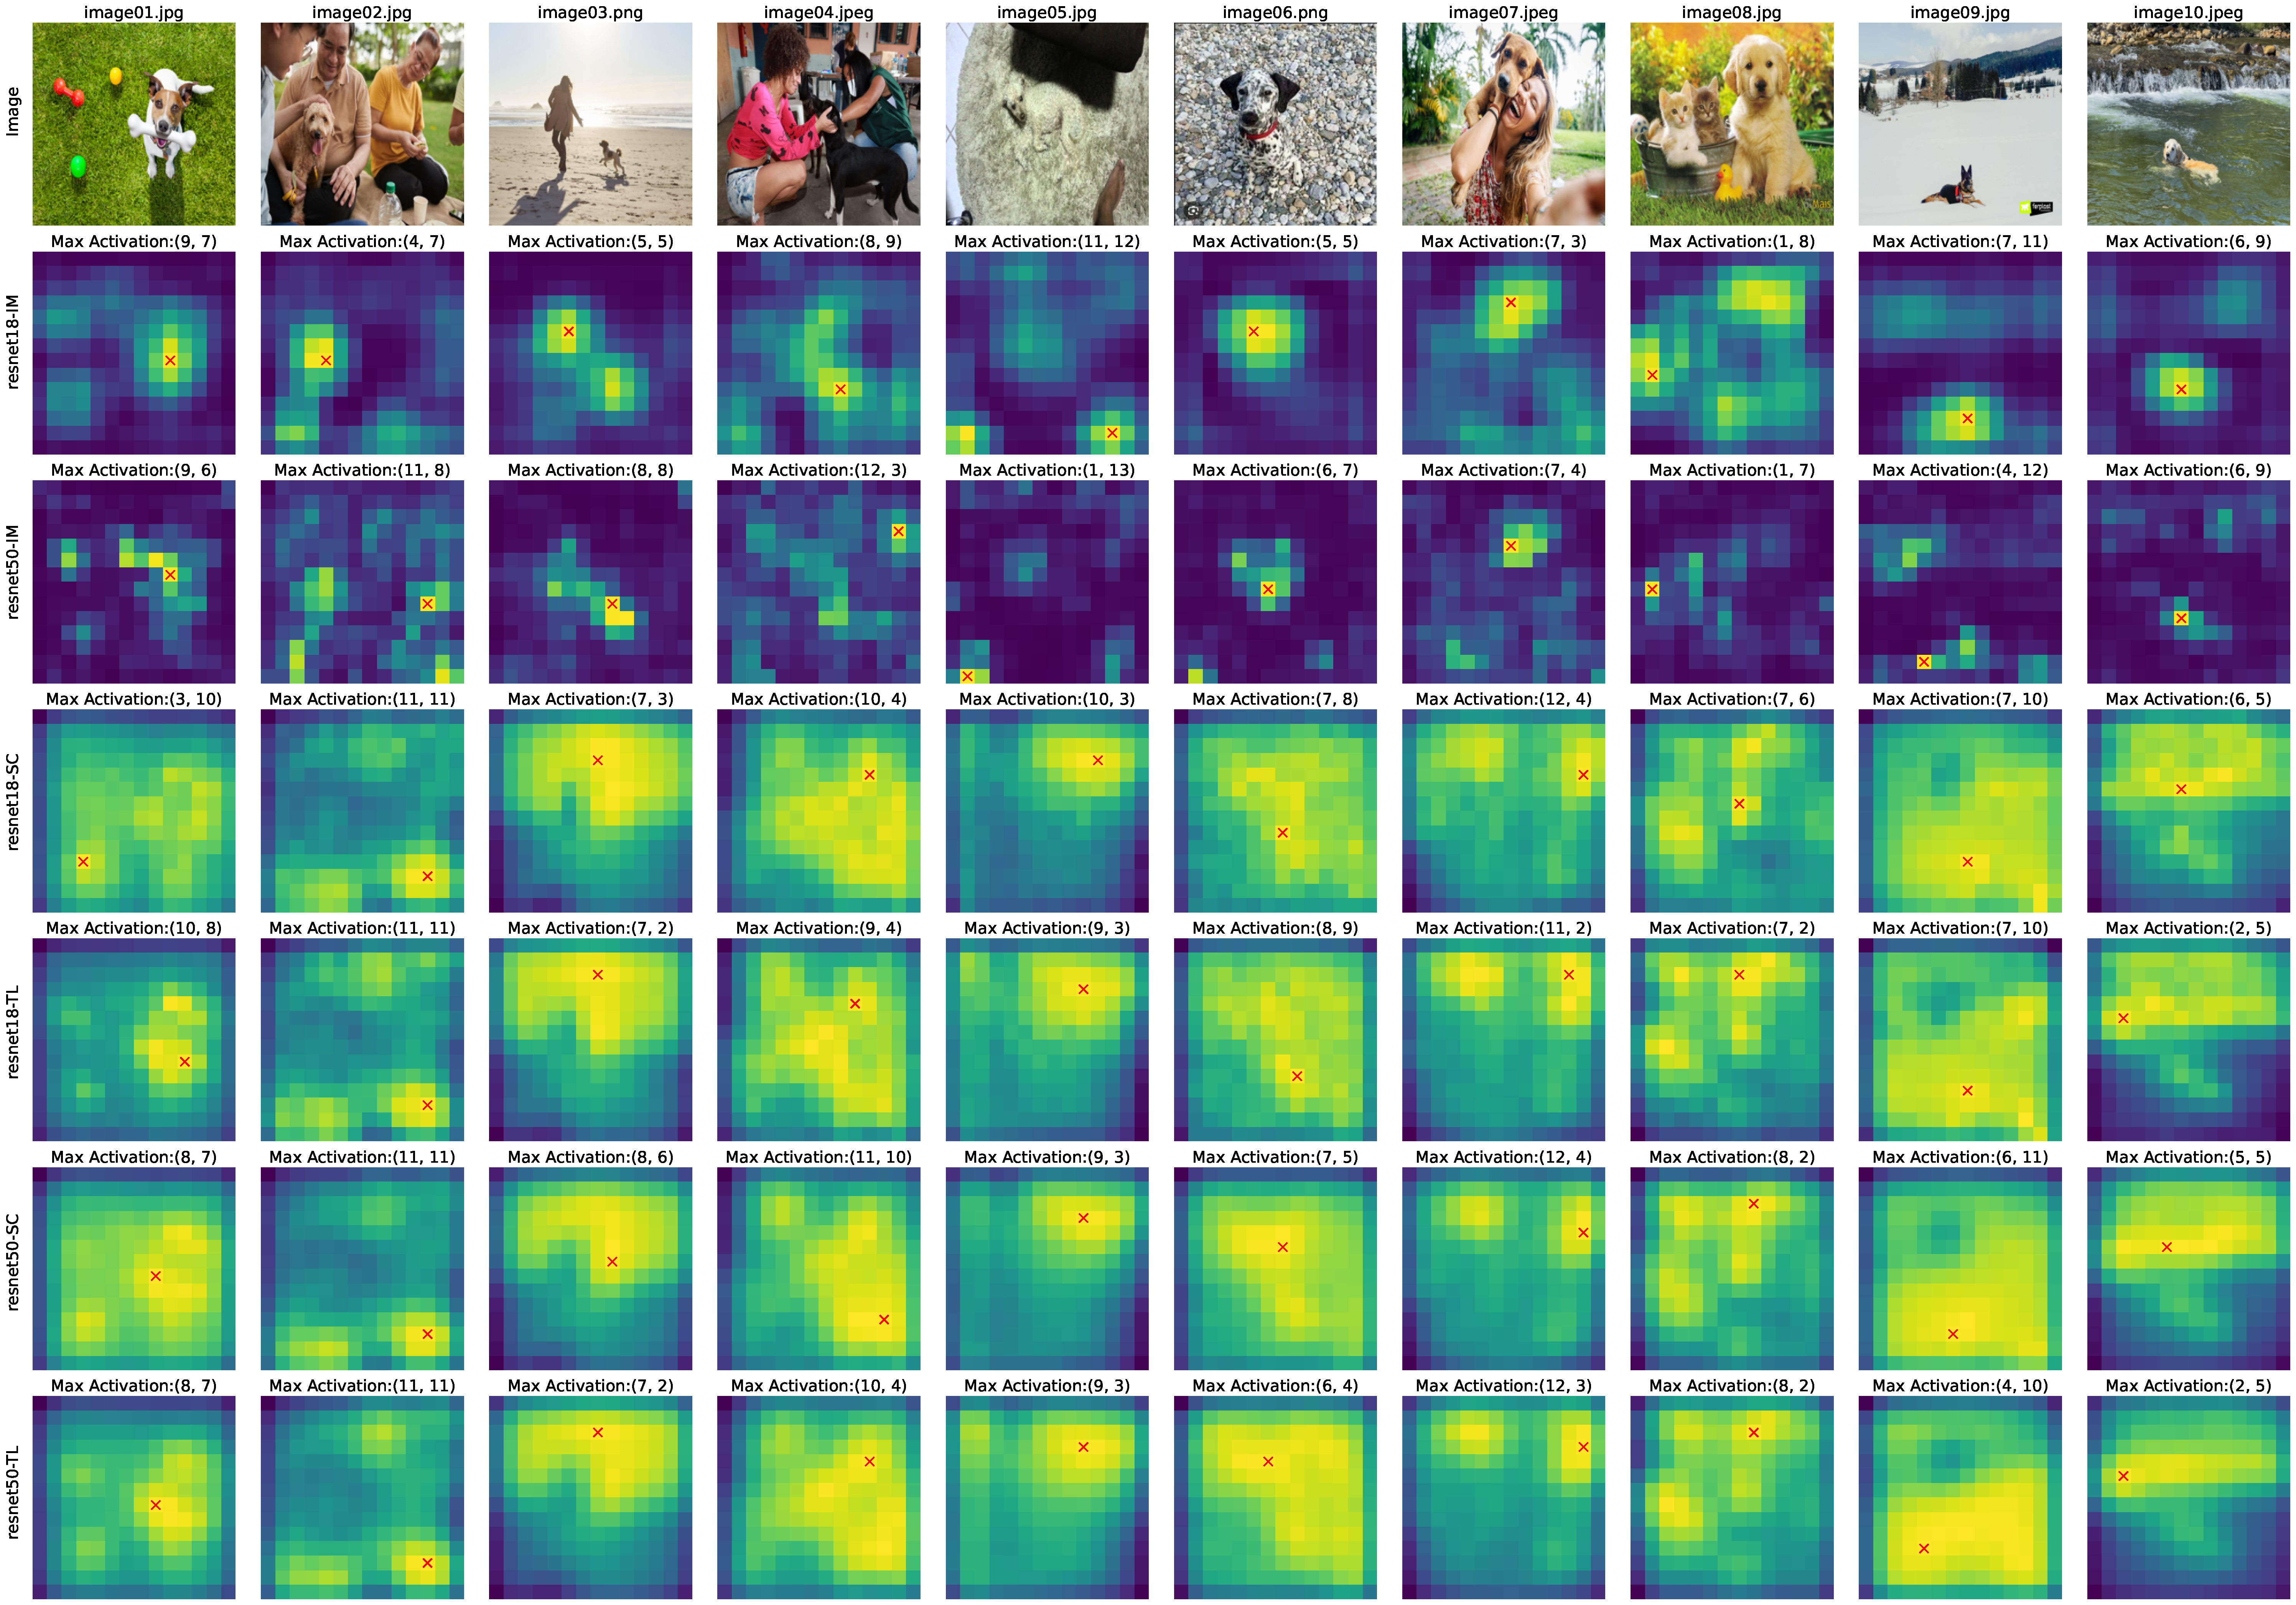
\includegraphics[width=0.98\textwidth]{imgs/activation_maps.pdf}
    \caption{Exemplo de mapas de ativação gerados pelos diferentes modelos.}
\end{figure*}

\begin{figure*}[htb]
    \centering
    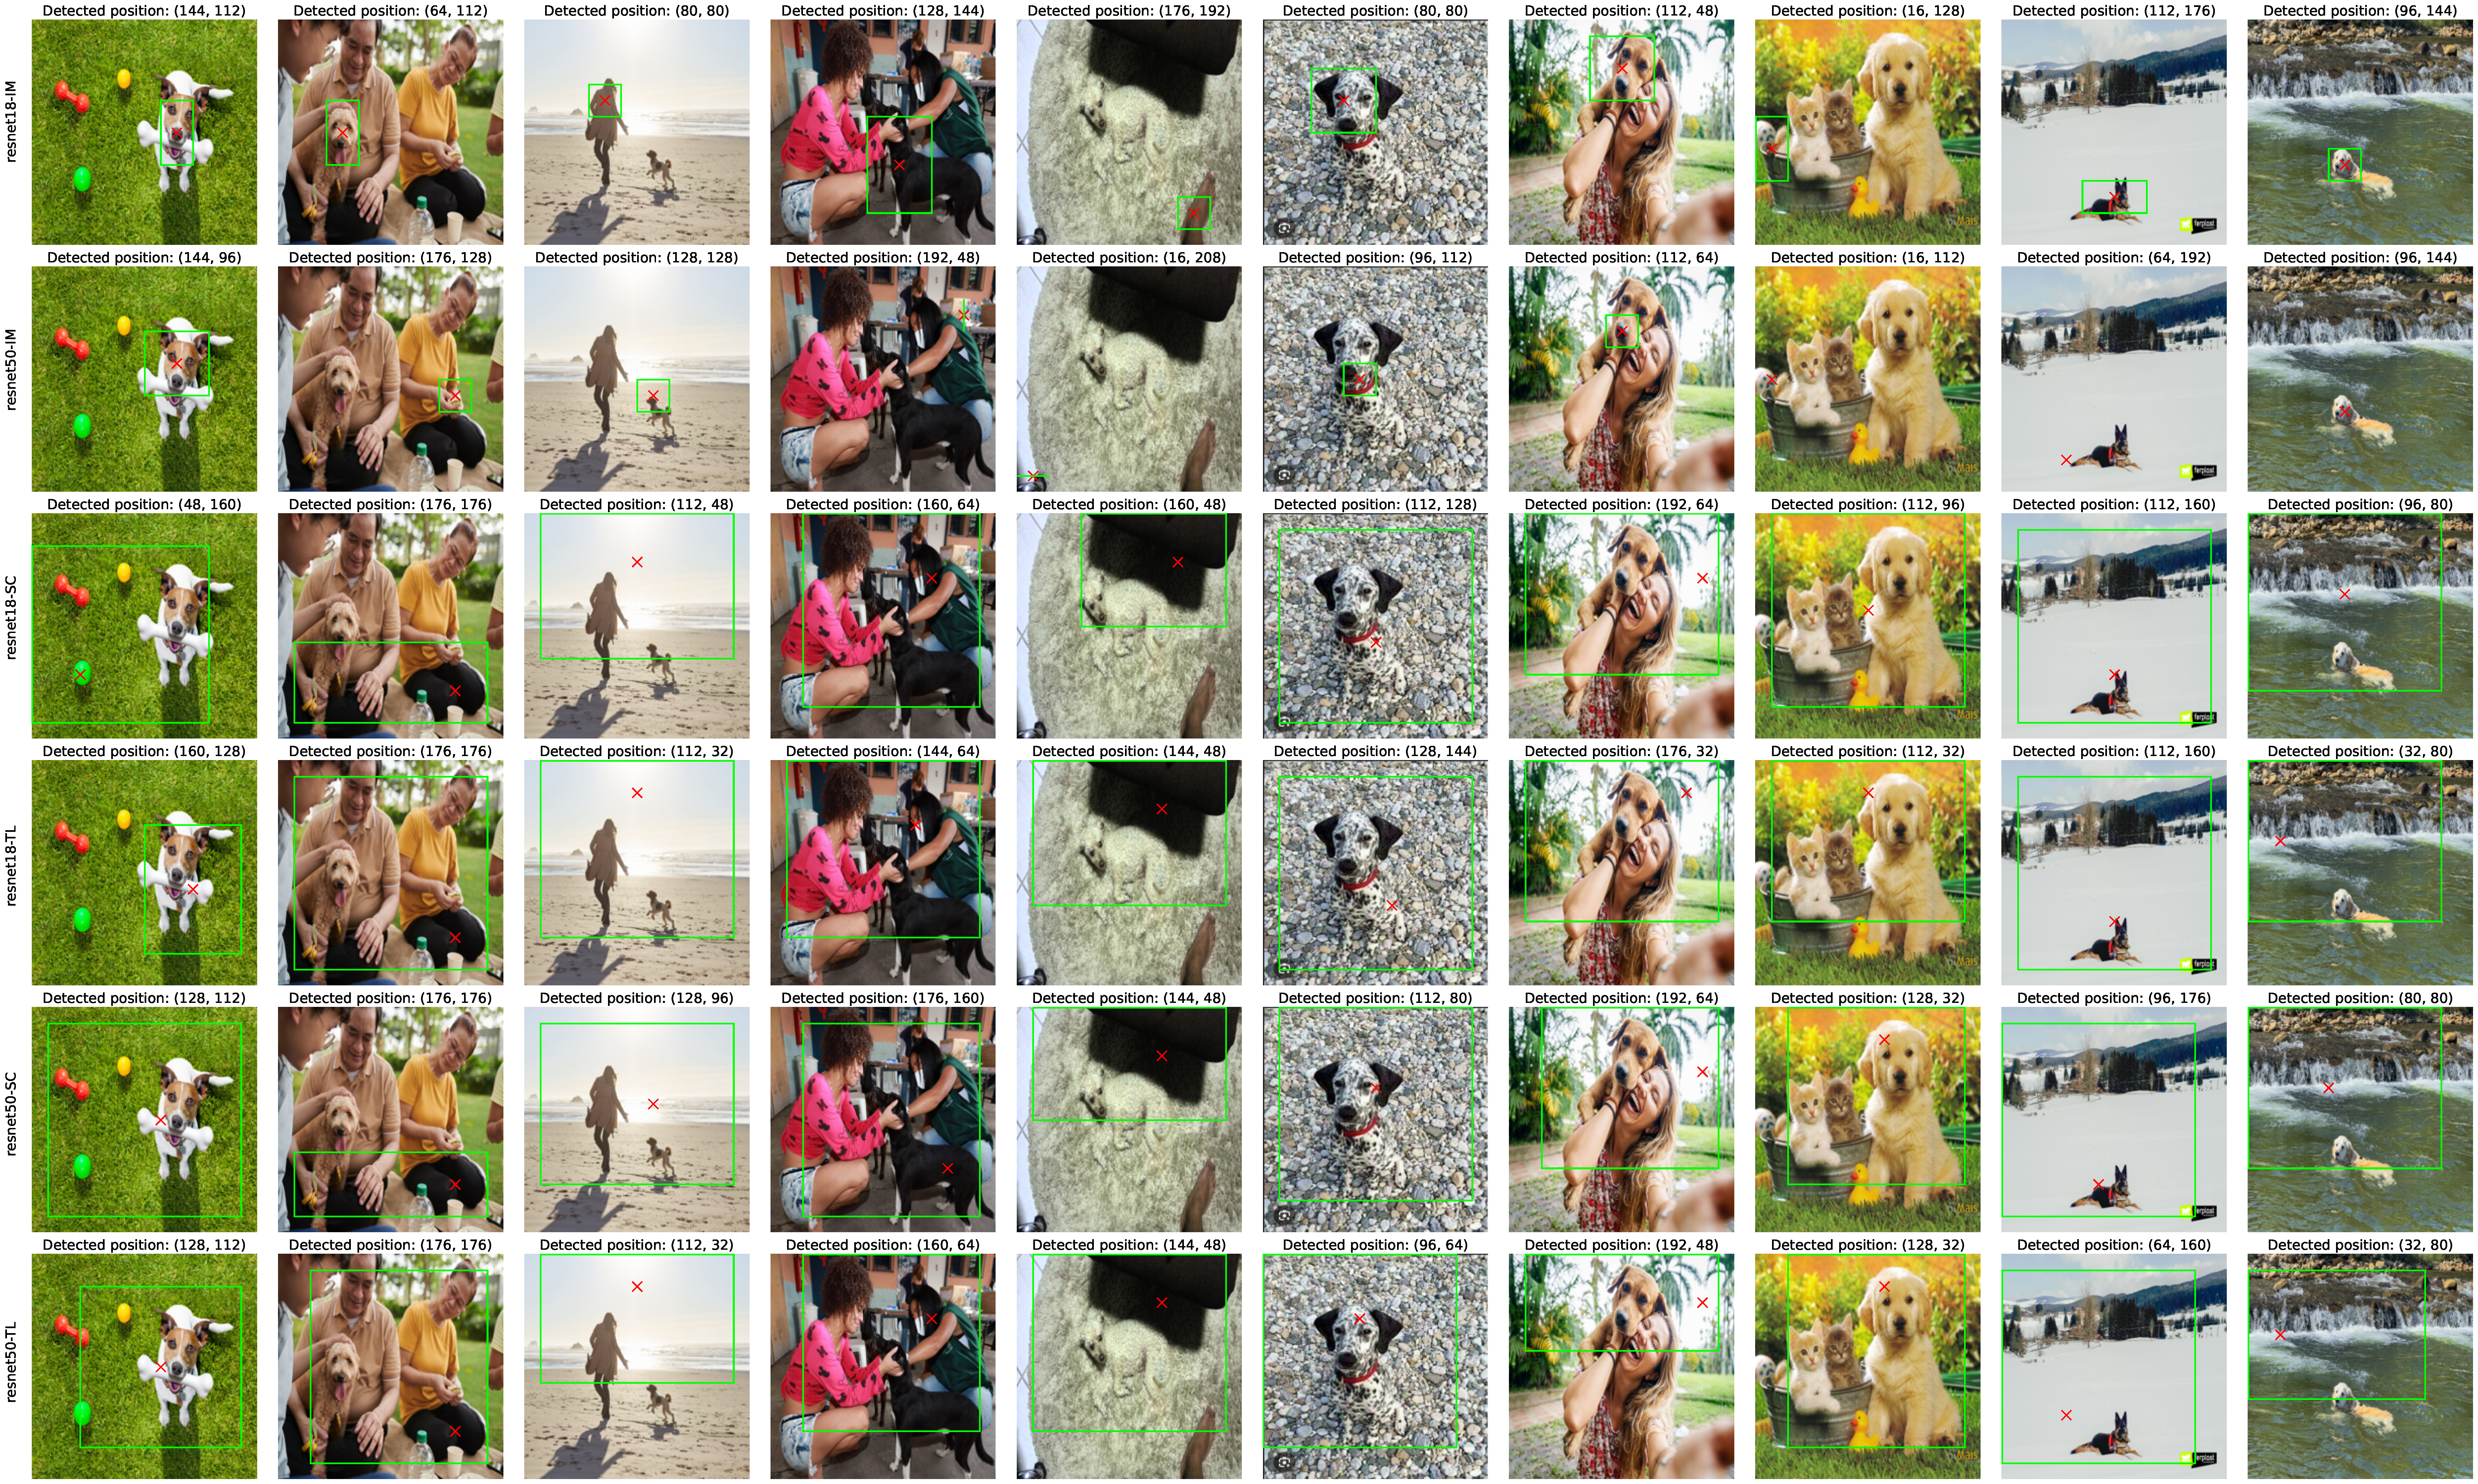
\includegraphics[width=0.98\textwidth]{imgs/detection_grid.pdf}
    \caption{Localização qualitativa dos cães nas imagens originais.}
\end{figure*}

\section{Conclusões}
O uso de mapas de ativação permite identificar regiões relevantes para a detecção de objetos, mesmo em cenários onde o objeto ocupa uma pequena parte da imagem. Modelos refinados apresentam desempenho superior, evidenciando a importância do ajuste fino para o domínio de interesse. O método é promissor para aplicações que exigem interpretabilidade e localização precisa.

\bibliography{apssamp}

\end{document}
